\documentclass[11pt, a4paper]{article}
\usepackage[utf8]{inputenc}

\usepackage[margin=1in]{geometry} 
\usepackage{amsmath,amsthm,amssymb}
\usepackage[margin=1in]{geometry} 
\usepackage{amsmath,amsthm,amssymb}

\usepackage[slovene]{babel}
\usepackage{color}
\usepackage{graphicx}
\usepackage{amssymb}
\usepackage{amsmath}
\usepackage{mathtools}
\usepackage{commath}
\usepackage{ragged2e}
\usepackage[T1]{fontenc}
\usepackage[normalem]{ulem}
\usepackage{amsthm}
\usepackage{esvect}
\usepackage{float}
\usepackage{calrsfs}
\DeclareMathAlphabet{\pazocal}{OMS}{zplm}{m}{n}
\newcommand{\Ga}{\mathcal{G}}
\mathtoolsset{showonlyrefs} 

\newcommand\setItemnumber[1]{\setcounter{enumi}{\numexpr#1-1\relax}}


\newtheorem{theorem}{Trditev}[section]
\newtheorem{corollary}{Posledica}[section]
\newtheorem{lemma}[section]{Lema}
\theoremstyle{definition}
\newtheorem{definition}{Definicija}[section]
\theoremstyle{example}
\newtheorem{example}[section]{Primer}
\theoremstyle{izrek}
\newtheorem{izrek}[section]{Izrek}

\begin{document}
\begin{center}
\thispagestyle{empty}
\parskip=14pt%
\vspace*{3\parskip}%
\begin{Huge} Določanje Boltzmanove konstate \end{Huge}

By

Matic Tonin

ID No. (28181098)

Mentor 

(Rok Dolenec)

\rule{7cm}{0.4pt}

Pod okvirom:

FAKULTETE ZA FIZIKO IN MATEMATIKO, LJUBLJANA

1. 4. 2020

\end{center}
\pagebreak
\section{Naloga}
\begin{enumerate}
\item Izmerite kolektorski tok tranzistorja $I_C$ v odvisnosti od $U_{BE}$ pri treh temperaturah:
približno 15, 35 in 55 °C.
\item Dolocite razmerje e0/kB.
\item Izmerite temperaturno odvisnost kolektorskega toka tranzistorja pri dveh napetostih
UBE približno 0.5 in 0.58 V.
\end{enumerate}
\section{Postopek dela}
Najprej preverimo, če smo ustvarili pravilno vezavo, kot nam narekujejo navodila. Napetost $U_{BE}$ za prvi del vaje nastavimo približno na 0.5 V in pazimo, da naj največji tok ne preseže 10mA. Z mikroamperom merimo kolektorski tok ($I_C$). Tranzistor potopimo v Dewarjevo posodo, da dosežemo različne temperature. In nato merimo tok v na kolektorju v odvisnosti od napetosti. \\\medskip
Pri drugem delu vaje merimo temperaturno odvisnost od kolektorskega toka pri neki stalni napetosti $U_{BE}$. Najprej stabiliziramo za iskano vrednost temperaturo, nato pa izmerimo kolektorski tok $I_C$. Tok $I_1$ si izberemo poljubno, glede na našo meritev. Pri teh meritvah neposredno merimo saturacijski tok, katerega temperaturna odvisnost je podana z nastavkom:

$$I_S(T)= \alpha T^n e^{\frac{-E_g (T)}{k_B T}}$$

kjer sta $\alpha$ in n neodvisna od temperature, $E_g$ pa je širina energijske vrzeli, ki je odvisna od temperature. 
\section{Meritve}

\subsection{Meritev boltzmanove konstante}
Za to nalogo smo uporabljali N-P-N bipolarni tranzistor ki ima tri kontakte:
\begin{enumerate}
\item kolektor
\item emitor
\item baza
\end{enumerate}
ki so med seboj zvezani, kot prikazuje spodnja slika:
\begin{figure}[H]
    \centering
    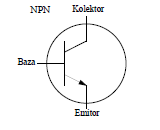
\includegraphics[width=7cm]{N-p-n.png}
    \caption{Prikaz n-p-n kolektorja}
\end{figure}

Tok, ki teče skozi kolektor je enak $I_C$, napetost, ki pa je med bazo in emitorjem pa zapišemo kot $U_{BE}$ 
Teoretična napoved je podana kot: 
$$I_{\mathrm{C}}=I_{\mathrm{S}}(T)\left[\exp \left(\frac{e_{0} U_{\mathrm{BE}}}{k_{\mathrm{B}} T}\right)-1\right]$$
ampak ker je eksponent dovolj večji kot 1 lahko to 1 zanemarimo in dobimo:
$$I_{\mathrm{C}}=I_{\mathrm{S}}(T)\exp \left(\frac{e_{0} U_{\mathrm{BE}}}{k_{\mathrm{B}} T}\right)$$

Ta relacija drži do 1 \% natančno.
\subsubsection{Temperatura 24°C}
Za ta del meritve smo morali najprej izmeriti tok na kolektorju v odvisnosti od višanje napetosti $U_{BE}$ pri neki stalni temperaturi, ki je bila v naši Dewarjevi posodi. Nato pa smo morali narisati funkcijo odvisnotsi $I_C$ od napetosti $U_{BE}$:
Dobili smo:
\begin{figure}[H]
    \centering
    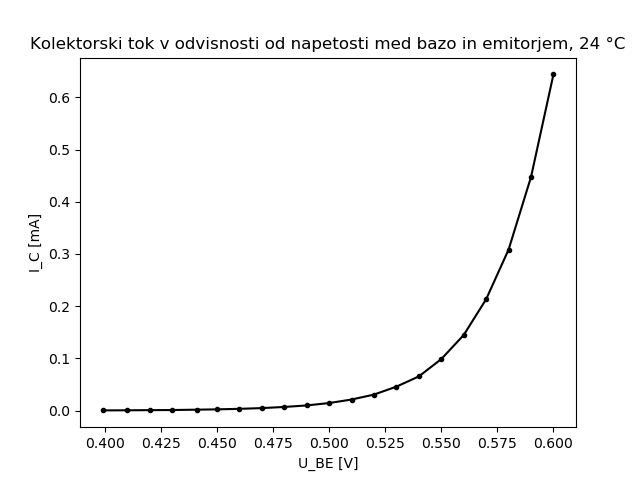
\includegraphics[width=10cm]{Napetost-tok,24.png}
    \caption{Prikaz odvisnosti toka na kolektorju od napetosti med bazo in emitorjem, 24 °C}
\end{figure}
Pri meritvi se lepo vidi eksponentno naraščanje, želimo pa videti odvisnost kot premico, podano z enačbo:

$$\ln(\frac{I_C}{I_1})=\ln(\frac{I_S(T)}{I_1})+\frac{e_0}{k_B T} U_{BE}$$
kjer bo naklon premice kar enak $\frac{e_0}{k_B T}$.
Če sedaj to narišemo, dobimo, da je:
\begin{figure}[H]
    \centering
    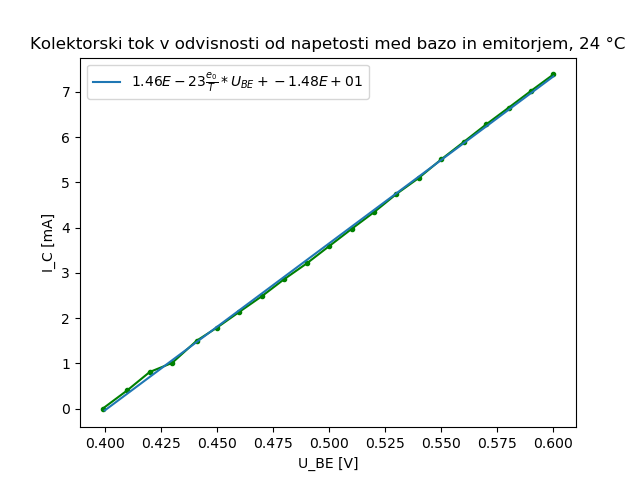
\includegraphics[width=10cm]{Napetost-tok_fit,24.png}
    \caption{Prikaz linearizacije podane eksponentne funkcije, 24 °C}
\end{figure}

V sam fit funkcije smo nastavili parametre tako, da nam v legendo avtomatsko izpiše vrednost boltzmanove konstante, ki jo pri temperaturi 20 °C dobimo:

$$k_B=1.46\cdot 10^{-23} \cdot \frac{J}{K} (1 \pm 0.06)$$
\subsubsection{Temperatura 43°C}
Za ta del meritve smo morali najprej izmeriti tok na kolektorju v odvisnosti od višanje napetosti $U_{BE}$ pri neki stalni temperaturi, ki je bila v naši Dewarjevi posodi. Nato pa smo morali narisati funkcijo odvisnotsi $I_C$ od napetosti $U_{BE}$:
Dobili smo:
\begin{figure}[H]
    \centering
    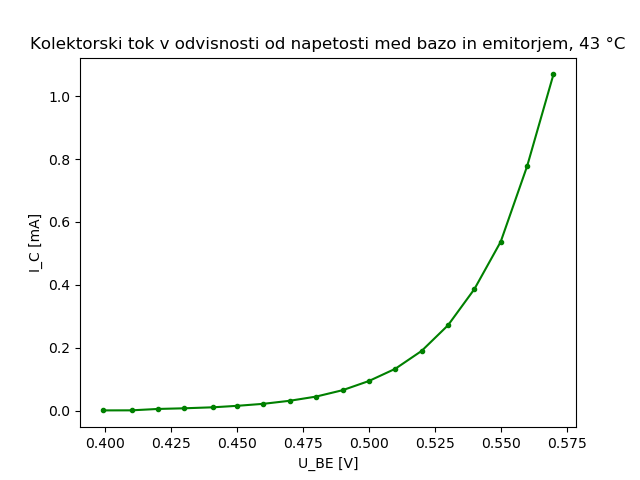
\includegraphics[width=10cm]{Napetost-tok,43.png}
    \caption{Prikaz odvisnosti toka na kolektorju od napetosti med bazo in emitorjem, 43 °C}
\end{figure}
Pri meritvi se lepo vidi eksponentno naraščanje in kot pri prejšnji nalogi, narišemo še premico, da odčitamo koeficient.
\begin{figure}[H]
    \centering
    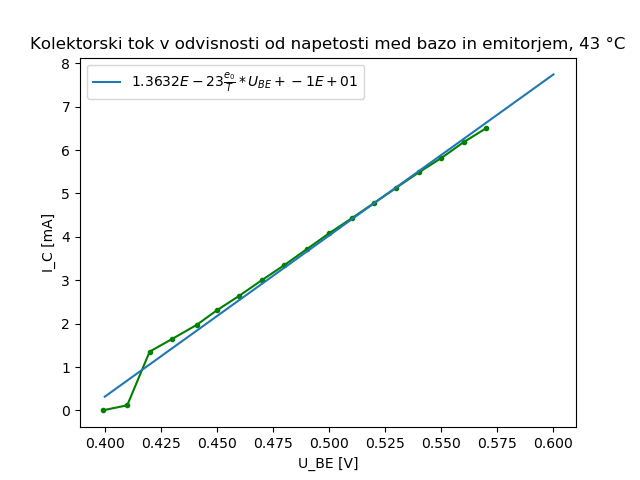
\includegraphics[width=10cm]{Napetost-tok_fit,43.png}
    \caption{Prikaz linearizacije podane eksponentne funkcije, 43 °C}
\end{figure}

V sam fit funkcije smo nastavili parametre tako, da nam v legendo avtomatsko izpiše vrednost boltzmanove konstante, ki jo pri temperaturi 20 °C dobimo:

$$k_B=1.363\cdot 10^{-23} \cdot \frac{J}{K} (1 \pm 0.06)$$

\subsubsection{Temperatura 60°C}
Za ta del meritve smo morali najprej izmeriti tok na kolektorju v odvisnosti od višanje napetosti $U_{BE}$ pri neki stalni temperaturi, ki je bila v naši Dewarjevi posodi. Nato pa smo morali narisati funkcijo odvisnotsi $I_C$ od napetosti $U_{BE}$:
Dobili smo:
\begin{figure}[H]
    \centering
    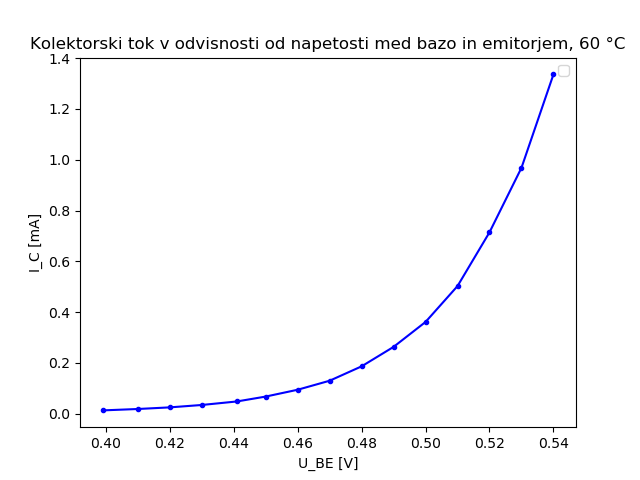
\includegraphics[width=10cm]{Napetost-tok,60.png}
    \caption{Prikaz odvisnosti toka na kolektorju od napetosti med bazo in emitorjem, 60 °C}
\end{figure}
Pri meritvi se lepo vidi eksponentno naraščanje, ponvno pa si želimo premice, zato skiciramo graf: 
\begin{figure}[H]
    \centering
    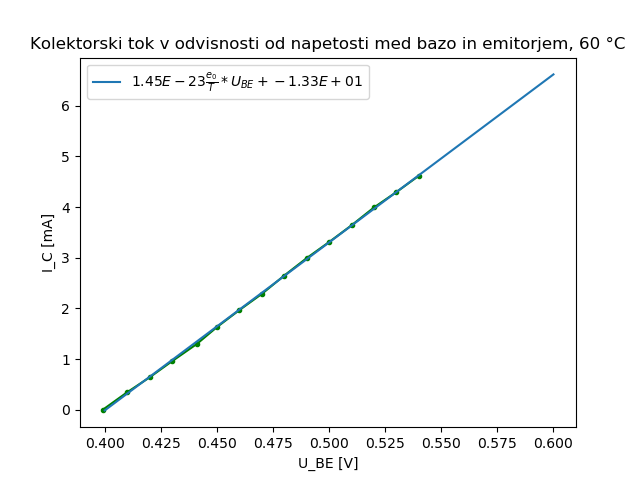
\includegraphics[width=10cm]{Napetost-tok_fit,60.png}
    \caption{Prikaz linearizacije podane eksponentne funkcije, 60 °C}
\end{figure}


V sam fit funkcije smo nastavili parametre tako, da nam v legendo avtomatsko izpiše vrednost boltzmanove konstante, ki jo pri temperaturi 20 °C dobimo:

$$k_B=1.45\cdot 10^{-23} \cdot \frac{J}{K} (1 \pm 0.06)$$

\subsubsection{Skupna vrednost boltzmanove konstante}
Če najprej vse vrednosti sestavimo v tabelo, dobimo da so: 

\begin{table}[H]
	\centering
	\begin{tabular}{|c|c|c|}
		\hline
		Temperatura  &  $k_B \quad [\frac{J}{K}]$ & $\overline{k_B}$\\
		\hline
		\hline
		20  & $1.46\cdot 10^{-23}$ & //\\
		\hline
		43  & $1.363\cdot 10^{-23}$ & //\\
		\hline
		60  & $1.45\cdot 10^{-23}$ & //\\
		\hline
		//&  // & $1.42 \cdot 10^{-23}$\\ 
		\hline
		\hline
	\end{tabular}
	\caption{Podatki o meritvah boltzmanove konstante}	
\end{table}

Vidimo, da je povprečna vrednost naše izračunane boltzmanove konstante enaka:

$$\underline{\underline{k_B=1.42 \cdot 10^{-23}\cdot \frac{J}{K} (1 \pm 0.06)}}$$

\pagebreak
\subsection{Meritev odvisnosti kolektorskega toka}
Če sedaj ponovimo postopek pri prejšnjih vajah, le da tokrat namesto napetosti spreminjamo temperauro, dobimo meritve. 
\subsubsection{Napetost 0.5 V}
Če najprej narišemo zgolj graf odvisnosti toka od temperature, dobimo, da je: 
\begin{figure}[H]
    \centering
    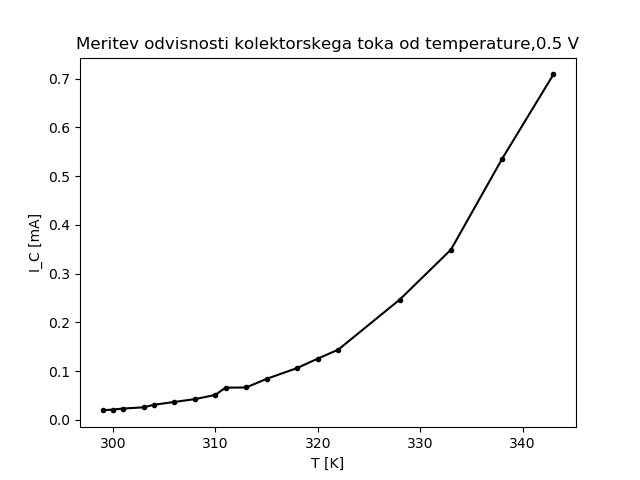
\includegraphics[width=10cm]{Napetost-temperatura,0,5.png}
    \caption{Prikaz odvisnotsi toka na kolektorju od temperature tranzistorja, 0,5 V}
\end{figure}
Če ponovno lineariziramo to funkcijo, dobimo premico in sicer.
\begin{figure}[H]
    \centering
    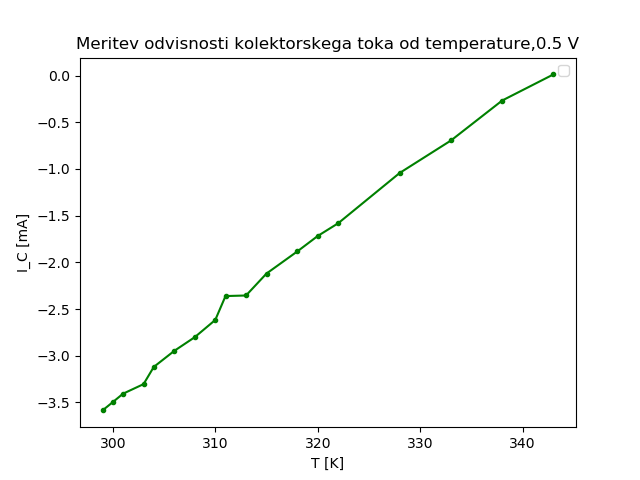
\includegraphics[width=10cm]{Napetost-temperatura_fut,0,5.png}
    \caption{Prikaz linearizacije podane eksponentne funkcije, 0.57 V}
\end{figure}


\subsubsection{Napetost 0.57 V}
Če najprej narišemo zgolj graf odvisnosti toka od temperature, dobimo, da je: 
\begin{figure}[H]
    \centering
    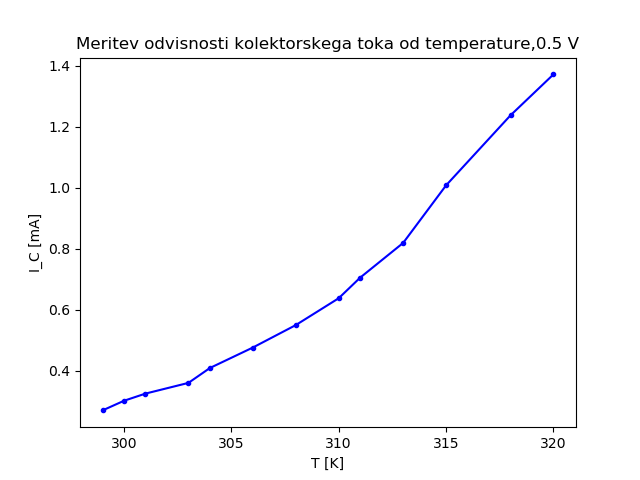
\includegraphics[width=10cm]{Napetost-temperatura,0,57.png}
    \caption{Prikaz odvisnotsi toka na kolektorju od temperature tranzistorja, 0.57 V}
\end{figure}

Ta graf zaenkrat še ne pokaže eksponentne odvisnosti, ampak, če to ponovno lineariziramo, kot smo to pri prejšnjem delu naredili, dobimo lepo linearno funkcijo:
\begin{figure}[H]
    \centering
    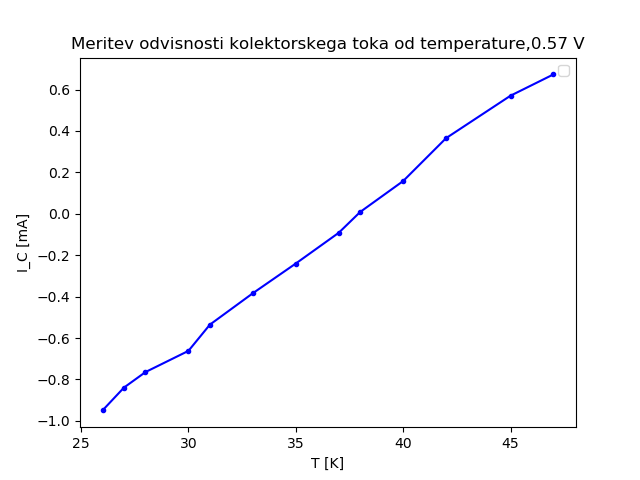
\includegraphics[width=10cm]{Napetost-temperatura_fut,0,57.png}
    \caption{Prikaz linearizacije podane eksponentne funkcije, 0.57 V}
\end{figure}

\end{document}